\section{The Fundamental Theorem of Calculus, Part I} \label{S:4.4.FTCI}

\begin{goals}
\item Given a function $f$, how does the rule $\ds A(x) = \int_a^x f(t) \, dt$ define a new function $A$?
\item What is the statement of the Fundamental Theorem of Calculus, and how do we apply the theorem?
\end{goals}

%-----------------------------------
% SUBSECTION INTRODUCTION
%-----------------------------------
\subsection*{Introduction}

\begin{marginfigure}[2.5in] % MARGIN FIGURE
\margingraphics{figs/4/4-4_Areafb.pdf}
\caption{A function $f$ and its corresponding area function $A(x) = \int_0^x f(t) \ dt$.} \label{fig:4-4_Areaf}
\end{marginfigure}

Given a continuous function $f$ defined on $[a,b]$, we define the corresponding integral, or area, function $A$ according to the rule 
\begin{equation} \label{E:intfxn}
A(x) = \int_a^x f(t) \, dt.
\end{equation}
Note particularly that because we are using the variable $x$ as the independent variable in the function $A$, and $x$ determines the other endpoint of the interval over which we integrate (starting from $a$), we need to use a variable other than $x$ as the variable of integration.  A standard choice is $t$, but any variable other than $x$ is acceptable.

One way to think of the function $A$ is as the ``net-signed area from $a$ up to $x$'' function, where we consider the region bounded by $y = f(t)$ on the relevant interval.  For example, in Figure~\ref{fig:4-4_Areaf}, we see a given function $f$ and its corresponding area function (choosing $a = 0$), $A(x) = \int_0^x f(t) \ dt$.

\begin{marginfigure} % MARGIN FIGURE
\captionsetup[subfigure]{labelformat=empty}
\subfloat{\margingraphics{figs/4/4-4_Areaf2a.pdf}}

\subfloat{\margingraphics{figs/4/4-4_Areaf2b.pdf}}
\caption{The area under $f$ and the height of $A(x)$.} \label{fig:4-4_Areaf2a}
\end{marginfigure}

Note particularly that the function $A$ measures the net-signed area from $t = 0$ to $t = x$ bounded by the curve $y = f(t)$; this value is then reported as the corresponding height on the graph of $y = A(x)$---see Figure~\ref{fig:4-4_Areaf2a}.  It is even more natural to think of this relationship between $f$ and $A$ dynamically.  At \href{http://gvsu.edu/s/cz}{\texttt{http://gvsu.edu/s/cz}}, we find a java applet that brings this relationship to life.  There, the user can move the red point on the function $f$ and see how the corresponding height changes at the light blue point on the graph of $A$.

\begin{pa} \label{PA:4.4}
Consider the function $A$ defined by the rule
\[ A(x) = \int_1^x f(t) \ dt, \]
where $f(t) = 4-2t$ as seen in Figure~\ref{fig:preview_4-4}.

\ba
\item Compute $A(1)$ and $A(2)$ exactly using geometry.

\item Suppose that we can produce a formula for $A(x)$ that does not use integrals, and suppose that formula is $\ds A(x) = -x^2 + 4x - 3$.  Observe that $f$ is a linear function; what kind of function is this additional formula for $A$?
%Use the First Fundamental Theorem of Calculus to find an equivalent formula for $A(x)$ that does not involve integrals.  That is, use the first FTC to evaluate $\int_1^x (4-2t) \, dt$.

%\item Observe that $f$ is a linear function; what kind of function is $A$?

\item Using the additional formula for $A(x)$ found in (b) that does not involve integrals, compute $A(1)$, $A(2)$, and $A'(x)$.

\item While we have defined $f$ by the rule $f(t) = 4-2t$, it is equivalent to say that $f$ is given by the rule $f(x) = 4 - 2x$.  What do you observe about the relationship between $A$ and $f$?
\ea
\end{pa}
\begin{marginfigure}[-3cm] % MARGIN FIGURE
\margingraphics{figs/4/preview_4-4.pdf}
\caption{$f(t) = 4-2t$} \label{fig:preview_4-4}
\end{marginfigure} 
\afterpa % PREVIEW ACTIVITY

The choice of the lower bournd of integration $a$ is somewhat arbitrary.  In the activity that follows, we explore how the value of $a$ affects the graph of the integral function, as well as some additional related issues.

\begin{marginfigure} % MARGIN FIGURE
\margingraphics{figs/4/activity_4-4-1a.pdf}
\caption{$y = g(t)$} \label{fig:activity_4-4-1a}
\end{marginfigure}

\begin{marginfigure} % MARGIN FIGURE
\margingraphics{figs/4/activity_4-4-1b.pdf}
\caption{Sketch $A(x) = \int_1^x g(t) \ dt$} \label{fig:activity_4-4-1b}
\end{marginfigure}

\begin{activity} \label{A:4.4.2}  
Suppose that $g$ is given by the graph at left in Figure~\ref{fig:activity_4-4-1a} and that $A$ is the corresponding integral function defined by $A(x) = \int_1^x g(t) \, dt$.
\ba
	\item On what interval(s) is $A$ an increasing function?  On what intervals is $A$ decreasing?  Why?
	\item On what interval(s) do you think $A$ is concave up?  concave down?  Why?
	\item At what point(s) does $A$ have a relative minimum?  a relative maximum?
	\item Use the given information to determine the exact values of $A(0)$, $A(1)$, $A(2)$, $A(3)$, $A(4)$, $A(5)$, and $A(6)$.
	\item Based on your responses to all of the preceding questions, sketch a complete and accurate graph of $y = A(x)$ on the axes provided, being sure to indicate the behavior of $A$ for $x < 0$ and $x > 6$.
	\item How does the graph of $B$ compare to $A$ if $B$ is instead defined by $B(x) = \int_0^x g(t) \, dt$?
\ea

\end{activity}
\begin{smallhint}
 \ba
	\item Where is $A$ accumulating positive signed area?	
	\item As $A$ accumulates positive or negative signed area, where is the rate at which such area is accumulated increasing?
	\item Where does $A$ change from accumulating positive signed area to accumulating negative signed area?
	\item Note, for instance, that $A(2) = \int_1^2 g(t) \, dt$.
	\item Use your work in (a)-(d) appropriately.
	\item What is the value of $B(0)$?  How does this compare to $A(0)$?
\ea
\end{smallhint}
\begin{bighint}
 \ba
	\item Where is $A$ accumulating positive signed area? Where is $A$ accumulating negative signed area?
	\item As $A$ accumulates positive or negative signed area, where is the rate at which such area is accumulated increasing?  Contrast, for instance, the behavior of $A$ on the intervals $(0,1)$ and $(1,2)$.
	\item Where does $A$ change from accumulating positive signed area to accumulating negative signed area?  From negative to positive?
	\item Note, for instance, that $A(2) = \int_1^2 g(t) \, dt$, $A(0) = \int_1^0 g(t) \, dt$, and particularly that $A(1) = \int_1^1 g(t) \, dt = 0$.
	\item Use your work in (a)-(d) appropriately.
	\item What is the value of $B(0)$?  How does this compare to $A02)$?  What if we compare $B(1)$ and $A(1)$?
\ea
\end{bighint}
\begin{activitySolution}
\ba
	\item $A$ is accumulating positive signed area wherever $g$ is positive, and thus $A$ is increasing on $(0,1.5)$, $(4,6)$;  $A$ is accumulating negative signed area and therefore decreasing wherever $g$ is negative, which occurs on $(1.5,4)$.
	\item Here we want to consider where $A$ is changing at an increasing rate (concave up) or changing at a decreasing rate (concave down).  On $(0,1)$ and $(4,5)$, $A$ is increasing, and we can also see that since $g$ is increasing, $A$ is increasing at an increasing rate.  Similarly, on $(3,4)$ (where $g$ is negative so $A$ is decreasing), since $g$ is increasing it follows that $A$ is decreasing at an increasing rate.  Thus, $A$ is concave up on $(0,1)$ and $(3,5)$.  Analogous reasoning shows that $A$ is concave down on $(1,3)$ and $(5,6)$.
	\item Based on our work in (a), we see that $A$ changes from increasing to decreasing at $x = 1.5$, and thus $A$ has a relative maximum there.  Similarly, $A$ has a relative minimum at $x = 4$.
	\item Using the fact that $g$ is piecewise linear and the definition of $A$, we find that $A(0) = \int_1^0 g(t) \, dt = -\int_0^1 g(t) \, dt = -\frac{1}{2}$; $A(1) = \int_1^1 g(t) \, dt = 0$; $A(2) = \int_1^2 g(t) \, dt = 0$.  Analogous reasoning shows that $A(3) = -2$, $A(4) = -3.5$, $A(5) = -2$, $A(6) = -0.5$.
	\item Use your work in (a)-(d) appropriately.
	\item Note that $B(0) = 0$, while $A(0) = -\frac{1}{2}$.  Likewise, $B(1) = \frac{1}{2}$, while $A(1) = 0$.  Indeed, we can see that for any value of $x$, $B(x) = A(x) + \frac{1}{2}$.
\ea
\end{activitySolution}
\aftera % ACTIVITY %change to not do FTCII

%--------------------------------------------------------------------
% SUBSECTION THE FUNDAMENTAL THEOREM OF CALCULUS
%--------------------------------------------------------------------
\subsection*{The Fundamental Theorem of Calculus} \index{fundamental theorem of calculus}

We can also apply calculus ideas to $A(x)$; in particular, we can compute its derivative. While this may seem like an innocuous thing to do, it has far--reaching implications, as demonstrated by the fact that the result is given as an important theorem.

\concept{Fundamental Theorem of Calculus, Part 1} % CONCEPT
{Let $f$ be continuous on $[a,b]$ and let $\ds A(x) = \int_a^x f(t)\ dt$. Then $A$ is a differentiable function on $(a,b)$, and\index{Fundamental Theorem of Calculus}\index{integration!Fun. Thm. of Calc.}
\[ A'(x)=f(x). \]
} % end concept

\proof In general, if $f$ is any continuous function, and we define the function $A$ by the rule 
\[ A(x) = \int_a^x f(t) \ dt, \]
where $a$ is an arbitrary constant, then we can show that $A$ is an antiderivative of $f$.  To see why, let's demonstrate that $A'(x) = f(x)$ by using the limit definition of the derivative.  Doing so, we observe that
\begin{align}
A'(x) &= \lim_{h \to 0} \frac{A(x+h) - A(x)}{h} \notag \\
&= \lim_{h \to 0} \frac{\int_a^{x+h} f(t) \, dt - \int_a^x f(t) \, dt}{h} \notag \\
&= \lim_{h \to 0} \frac{\int_x^{x+h} f(t) \, dt}{h}, \label{E:FTC2limdef}
\end{align}
where Equation~(\ref{E:FTC2limdef}) in the preceding chain follows from the fact that $\int_a^x f(t) \,dt + \int_x^{x+h} f(t) \, dt = \int_a^{x+h} f(t) \, dt$.  Now, observe that for small values of $h$,
\[ \int_x^{x+h} f(t) \ dt \approx f(x) \cdot h, \]
\begin{marginfigure} % MARGIN FIGURE
\margingraphics{figs/4/4-4_FTCh.pdf}
\caption{Approximating the area under $f$ from $x$ to $x+h$.} \label{fig:4-4_FTCh}
\end{marginfigure}
\noindent by a simple left-hand approximation of the integral. Thus, as we take the limit in Equation~(\ref{E:FTC2limdef}) as $h$ approaches $0$, it follows that
\[ A'(x) =  \lim_{h \to 0} \frac{\int_x^{x+h} f(t) \, dt}{h} = \lim_{h \to 0} \frac{f(x) \cdot h}{h} = f(x). \]
\qed

\begin{example} % EXAMPLE
Let $\ds A(x) = \int_{-5}^x  \left( t^2 + \sin(t) \right) \ dt$.  What is $A'(x)$?

\solution Using the Fundamental Theorem of Calculus, we have 
\[ A'(x) = x^2 + \sin(x). \]
\end{example} % EXAMPLE

\begin{example} % EXAMPLE
Let $\ds A(x) = \int_{\pi}^x \sin(t^2) \ dt$.  What is $A'(x)$?

\solution Using the Fundamental Theorem of Calculus, we have 
\[ A'(x) = \sin(x^2). \]
\end{example} % EXAMPLE

\begin{activity} \label{A:5.2.2}  Evaluate each of the following indefinite integrals.  

\bmtwo
\ba
	\item $\int \tan^3(x)\sec^2(x) \, dx$
	\item $\int \tan^4(x)\sec^4(x) \, dx$
	\item $\int \tan^3(x)\sec^3(x) \, dx $
	\item $\int \sin(6x)\sin(3x) \, dx $
\ea
\emtwo
\end{activity}
\begin{smallhint}
\ba
	\item Small hints for each of the prompts above.
\ea
\end{smallhint}
\begin{bighint}
\ba
	\item Big hints for each of the prompts above.
\ea
\end{bighint}
\begin{activitySolution}
\ba
	\item Solutions for each of the prompts above.
\ea
\end{activitySolution}
\aftera % ACTIVITY 

%-------------------------------------------------------------------------------------------
% SUBSECTION THE FUNDAMENT THEOREM AND THE CHAIN RULE
%-------------------------------------------------------------------------------------------
\subsection{The Fundamental Theorem and the Chain Rule}

The Fundamental Theorem of Calculus states that given $A(x) = \int_a^x f(t)\ dt$,  $A'(x) = f(x)$, or we can use other notation to write $\frac{d}{dx}\left[ A(x) \right] = f(x)$. It may be of further use to compose such a function with another. As an example, we may compose $A(x)$ with $g(x)$ to get 
\[ (A \circ g)(x) = \int_a^{g(x)} f(t) \ dt.\]
What is the derivative of such a function?\index{Fundamental Theorem of Calculus!and Chain Rule} Since it is a composition, the Chain Rule can be employed.  We decompose the composition as
\[ y = \int_a^u f(t) \ dt \quad \mbox{where} \quad u = g(x). \]
Using the Leibniz version of the Chain Rule, we have
\[ \frac{dy}{dx} = \frac{dy}{du} \cdot \frac{du}{dx}, \] 
where
\[ \frac{dy}{du} = f(u) \quad \mbox{and} \quad \frac{du}{dx} = g'(x). \]
Therefore,
\[ \frac{dy}{dx} = f(u) \cdot g'(x) = f \left( g(x) \right) \cdot g'(x). \]

\begin{example} % EXAMPLE
Using the FTC and the Chain Rule, compute the derivative of $\ds A(x) = \int_2^{x^2} \ln(t) \ dt$.

\solution Noticing that this function is a composition, we can decompose it as
\[ y = \int_2^u \ln(t) \ dt \quad \mbox{where} \quad u = x^2. \]
Using the Leibniz version of the Chain Rule, we have
\[ \frac{dy}{dx} = \frac{dy}{du} \cdot \frac{du}{dx}, \] 
where
\[ \frac{dy}{du} = \ln(u) \quad \mbox{and} \quad \frac{du}{dx} = 2x. \]
Therefore,
\[ \frac{dy}{dx} = \ln(u) \cdot 2x = \ln \left( x^2 \right) \cdot 2x. \]
\end{example} % EXAMPLE

\begin{example} % EXAMPLE 
Compute the derivative of $\ds A(x) = \int_{\cos(x)}^5 t^3\ dt.$

\solution Note that $\ds A(x) = -\int_5^{\cos(x)} t^3\ dt$, which is again a composition. We can decompose it as
\[ y = -\int_5^u t^3 \ dt \quad \mbox{where} \quad u = \cos(x). \]
Using the Leibniz version of the Chain Rule, we have
\[ \frac{dy}{dx} = \frac{dy}{du} \cdot \frac{du}{dx}, \] 
where
\[ \frac{dy}{du} = -u^3 \quad \mbox{and} \quad \frac{du}{dx} = -sin(x). \]
Therefore,
\[ \frac{dy}{dx} = -u^3 \cdot -sin(x) = \cos^3(x) \cdot \sin(x). \]
\end{example} % EXAMPLE

\begin{activity} \label{A:5.2.2}  Evaluate each of the following indefinite integrals.  

\bmtwo
\ba
	\item $\int \tan^3(x)\sec^2(x) \, dx$
	\item $\int \tan^4(x)\sec^4(x) \, dx$
	\item $\int \tan^3(x)\sec^3(x) \, dx $
	\item $\int \sin(6x)\sin(3x) \, dx $
\ea
\emtwo
\end{activity}
\begin{smallhint}
\ba
	\item Small hints for each of the prompts above.
\ea
\end{smallhint}
\begin{bighint}
\ba
	\item Big hints for each of the prompts above.
\ea
\end{bighint}
\begin{activitySolution}
\ba
	\item Solutions for each of the prompts above.
\ea
\end{activitySolution}
\aftera % ACTIVITY

%--------------------------------------------------------------------
% SUBSECTION UNDERSTANDING INTEGRAL FUNCTIONS
%--------------------------------------------------------------------
\subsection*{Understanding Integral Functions}%\index{}\index{}

The FTC provides us with a means to construct an antiderivative of any continuous function.  In particular, if we are given a continuous function $g$ and wish to find an antiderivative of $G$, we can now say that 
\[ G(x) = \int_c^x g(t) \ dt \]
provides the rule for such an antiderivative, and moreover that $G(c) = 0$.  Note especially that we know that $G'(x) = g(x)$.  We sometimes want to write this relationship between $G$ and $g$ from a different notational perspective.  In particular, observe that
\begin{equation} \label{E:diffint}
\frac{d}{dx} \left[ \int_c^x g(t) \, dt \right] = g(x).
\end{equation}
This result can be particularly useful when we're given an integral function such as $G$ and wish to understand properties of its graph by recognizing that $G'(x) = g(x)$, while not necessarily being able to exactly evaluate the definite integral $\int_c^x g(t) \ dt$.  

To see how this is the case, let's investigate the behavior of the integral function 
\[ E(x) = \int_0^x e^{-t^2} \ dt. \]
$E$ is closely related to the well known \emph{error function}\index{error functin}\footnote{The error function is defined by the rule $\ds \mbox{erf}(x)~=~\frac{2}{\sqrt{\pi}} \int_0^x e^{-t^2} \,dt$ and has the key property that $0 \le \mbox{erf}(x) < 1$ for all $x \ge 0$ and moreover that $\ds \lim_{x \to \infty} \mbox{erf}(x) = 1$.}, a function that is particularly important in probability and statistics.  It turns out that the function $e^{-t^2}$ does not have an elementary antiderivative that we can express without integrals.  That is, whereas a function such as $f(t) = 4-2t$ has elementary antiderivative $F(t) = 4t - t^2$, we are unable to find a simple formula for an antiderivative of $e^{-t^2}$ that does not involve a definite integral.  We will learn more about finding (complicated) algebraic formulas for antiderivatives without definite integrals in the chapter on infinite series.

Returning our attention to the function $E$, while we cannot evaluate $E$ exactly for any value other than $x = 0$, 
we still can gain a tremendous amount of information about the function $E$.  To begin, applying the rule in Equation~(\ref{E:diffint}) to $E$, it follows that
\[ E'(x) = \frac{d}{dx} \left[ \int_0^x e^{-t^2} \ dt \right] = e^{-x^2}, \]
so we know a formula for the derivative of $E$.  Moreover, we know that $E(0) = 0$.  This information is precisely the type we were given in problems such as the one in Activity~\ref{A:3.2.1} and others in Section~\ref{S:3.2.Tests}, where we were given information about the derivative of a function, but lacked a formula for the function itself.  

Here, using the first and second derivatives of $E$, along with the fact that $E(0) = 0$, we can determine more information about the behavior of $E$.  First, with $E'(x) = e^{-x^2}$, we note that for all real numbers $x$, $e^{-x^2} > 0$, and thus $E'(x) > 0$ for all $x$.  Thus $E$ is an always increasing function.  Further, we note that as $x \to \infty$, $E'(x) = e^{-x^2} \to 0$, hence the slope of the function $E$ tends to zero as $x \to \infty$ (and similarly as $x \to -\infty$).  This tells us that $E$ has horizontal asymptotes as $x$ increases or decreases without bound. 

In addition, we can observe that $E''(x) = -2xe^{-x^2}$, and that $E''(0) = 0$, while $E''(x) < 0$ for $x > 0$ and $E''(x) > 0$ for $x < 0$.  This information tells us that $E$ is concave up for $x<0$ and concave down for $x > 0$ with a point of inflection at $x = 0$.  

The only thing we lack at this point is a sense of how big $E$ can get as $x$ increases.  If we use a midpoint Riemann sum with 10 subintervals to estimate $E(2)$, we see that $E(2) \approx 0.8822$; a similar calculation to estimate $E(3)$ shows little change ($E(3) \approx 0.8862$), so it appears that as $x$ increases without bound, $E$ approaches a value just larger than $0.886$.  Putting all of this information together (and using the symmetry of $f(t) = e^{-t^2}$), we see the results shown in Figure~\ref{fig:4-4_erfa}.

\begin{marginfigure}[-4cm] % MARGIN FIGURE
\captionsetup[subfigure]{labelformat=empty}
\subfloat{\margingraphics{figs/4/4-4_erfa.pdf}}

\subfloat{\margingraphics{figs/4/4-4_erfb.pdf}}
\caption{At top, the graph of $f(t) = e^{-t^2}$.  At bottom, the integral function $E(x) = \int_0^x e^{-t^2} \,dt$, which is the unique antiderivative of $f$ that satisfies $E(0) = 0$.} \label{fig:4-4_erfa}
\end{marginfigure}

Again, $E$ is the antiderivative of $f(t) = e^{-t^2}$ that satisfies $E(0) = 0$.  Moreover, the values on the graph of $y = E(x)$ represent the net-signed area of the region bounded by $f(t) = e^{-t^2}$ from $0$ up to $x$.  We see that the value of $E$ increases rapidly near zero but then levels off $x$ increases since there is less and less additional accumulated area bounded by $f(t) = e^{-t^2}$ as $x$ increases.

\begin{activity} \label{A:5.2.2}  Evaluate each of the following indefinite integrals.  

\bmtwo
\ba
	\item $\int \tan^3(x)\sec^2(x) \, dx$
	\item $\int \tan^4(x)\sec^4(x) \, dx$
	\item $\int \tan^3(x)\sec^3(x) \, dx $
	\item $\int \sin(6x)\sin(3x) \, dx $
\ea
\emtwo
\end{activity}
\begin{smallhint}
\ba
	\item Small hints for each of the prompts above.
\ea
\end{smallhint}
\begin{bighint}
\ba
	\item Big hints for each of the prompts above.
\ea
\end{bighint}
\begin{activitySolution}
\ba
	\item Solutions for each of the prompts above.
\ea
\end{activitySolution}
\aftera

%-------------
% SUMMARY
%-------------
\begin{summary} 
\item Given a function $f$, the rule $A(x) = \int_a^x f(t) \ dt$ defines a new function $A$ that measures the net-signed area bounded by $f$ on the interval $[a,x]$.  We call the function $A$ the integral function corresponding to $f$.

\item The Fundamental Theorem of Calculus part I is the following:  if $f$ is a continuous function and $a$ is any constant, then $A(x) = \int_a^x f(t) \ dt$ is the unique antiderivative of $f$ that satisfies $A(c) = 0$.

\item The Chain Rule can be applied to functions of the form: $F\big( g(x) \big) = \int_a^{g(x)} f(t) \ dt$.   
\[ \frac{d}{dx} \Big( F \big( g(x) \big) \Big) = F' \big( g(x) \big) g'(x) = f \big( g(x) \big) g'(x).\]
\end{summary}

\clearpage

%--------------
% EXERCISES
%--------------
\begin{adjustwidth*}{}{-2.25in}
\textbf{{\large Exercises}}
\setlength{\columnsep}{25pt}
\begin{multicols*}{2}
\noindent {\normalsize Problems} \small

\begin{enumerate}[1)]
% ITEM 
\item Let $g$ be the function pictured below at left, and let $F$ be defined by $F(x) = \int_{2}^x g(t) \, dt.$ Assume that the shaded areas have values $A_1 = 4.3$, $A_2 = 12.7$, $A_3 = 0.4$, and $A_4 = 1.8$.  Assume further that the portion of $A_2$ that lies between $x = 0.5$ and $x = 2$ is $5.4$.  
  
Sketch a carefully labeled graph of $F$ on the axes provided, and include a written analysis of how you know where $g$ is zero, increasing, decreasing, CCU, and CCD. 
 
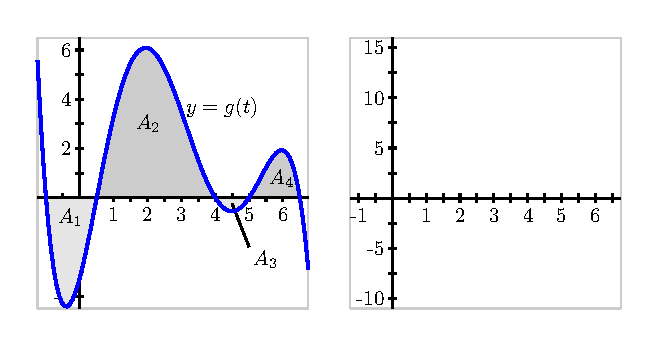
\includegraphics[scale=.75]{figures/5_2_Ez1.eps}

%ITEM
\item The tide removes sand from the beach at a small ocean park at a rate modeled by the function $$R(t) = 2 + 5\sin \left( \frac{4\pi t}{25} \right)$$
A pumping station adds sand to the beach at rate modeled by the function
$$S(t) = \frac{15t}{1+3t}$$
Both $R(t)$ and $S(t)$ are measured in cubic yards of sand per hour, $t$ is measured in hours, and the valid times are $0 \le t \le 6$.  At time $t = 0$, the beach holds $2500$ cubic yards of sand.

	\ba
		\item What definite integral measures how much sand the tide will remove during the time period $0 \le t \le 6$?  Why? 
		\item Write an expression for $Y(x)$, the total number of cubic yards of sand on the beach at time $x$.  Carefully explain your thinking and reasoning.
		\item At what instantaneous rate is the total number of cubic yards of sand on the beach at time $t = 4$ changing?  
		\item Over the time interval $0 \le t \le 6$, at what time $t$ is the amount of sand on the beach least?  What is this minimum value?  Explain and justify your answers fully.
	\ea
	
%ITEM
\item When an aircraft attempts to climb as rapidly as
possible, its climb rate (in feet per minute) decreases as altitude
increases, because the air is less dense at higher altitudes.
Given below is a table showing performance data for a certain
single engine aircraft, giving its climb rate at various altitudes, where  $c(h)$ denotes the climb rate of the airplane at an altitude $h$.

\begin{center}
\scalebox{.9}{
  \begin{tabular}{|c||c|c|c|c|c|c|}%%c|c|c|c|c|}
    \hline
    $h$ (feet)& $0$ & $1000$ & $2000$ & $3000$ & $4000$ & $5000$ \\%&6000&7000&8000&9000&10,000\\
    \hline
    $c$ (ft/min)& $925$ & $875$ & $830$ & $780$ & $730$ & $685$ \\%&635&585&535&490&440\\
    \hline
    \hline
    $h$ (feet)& $6000$ & $7000$ & $8000$ & $9000$ & $10,000$ &\\
    \hline
    $c$ (ft/min)& $635$ & $585$ & $535$ & $490$ & $440$ &\\
    \hline    
  \end{tabular}
} % end scalebox
\end{center}

 Let a new function $m$, that also depends on $h$, (say $y = m(h)$) measure
the number of minutes required for a plane at altitude $h$ to climb the
next foot of altitude.
\ba
	\item[a.] Determine a similar table of values for $m(h)$ and explain how it is related to the table above.  Be sure to discuss the units on $m$.

	\item[b.] Give a careful interpretation of a function whose derivative
is $m(h)$.  Describe what the input is and what the output is.  Also,
explain in plain English what the function tells us.

	\item[c.] Determine a definite integral whose value tells us exactly the number of minutes required for the airplane to ascend to
$10,000$ feet of altitude.  Clearly explain why the value of this integral has the required meaning.  

	\item[d.] Determine a formula for a function $M(h)$ whose value tells us the exact number of minutes required for the airplane to ascend to $h$ feet of altitude.

	\item[e.] Estimate the values of $M(6000)$ and $M(10000)$ as accurately as you can.  Include units on your results.
\ea
\end{enumerate}

\noindent{\bf In exercises 4--7, find $F'(x)$.}

\begin{enumerate}[1),resume]
\item $\ds F(x) = \int_2^{x^3+x} \frac{1}{t}\ dt$
\item $\ds F(x) = \int_{x^3}^{0} t^3\ dt$
\item $\ds F(x) = \int_{x}^{x^2} (t+2)\ dt$
\item $\ds F(x) = \int_{\ln x}^{e^x} \sin t\ dt$
\end{enumerate}

%------------------------------------------
% END OF EXERCISES ON FIRST PAGE
%------------------------------------------
\end{multicols*}
\end{adjustwidth*}

%\clearpage
%
%\begin{adjustwidth*}{}{-2.25in}
%\setlength{\columnsep}{25pt}
%\begin{multicols*}{2}\small
%
%\noindent{\bf In Exercises 69--72, an acceleration function of an object moving along a straight line is given. Find the change of the object's velocity over the given time interval.}
%
%\begin{enumerate}[1),start=69]
%\item $a(t) = -32$ ft/s$^2$ on $[0,2]$
%\item $a(t) = 10$ ft/s$^2$ on $[0,5]$
%\item $a(t) = t$ ft/s$^2$ on $[0,2]$
%\item $a(t) = \cos t$ ft/s$^2$ on $[0,\pi]$
%
%    \item A function $f$ is given piecewise by the formula
%  $$f(x) = \left\{ 
%  	\begin{array}{lr}
%	-x^2 + 2x + 1, & \ \mbox{if} \ 0 \le x < 2 \\
%	-x + 3, & \ \mbox{if} \ 2 \le x < 3 \\
%	x^2 - 8x + 15, & \ \mbox{if} \ 3 \le x \le 5
%	\end{array}
%	\right.
%  $$
%  \ba
%  	\item Determine the exact value of the net signed area enclosed by $f$ and the $x$-axis on the interval $[2,5]$.
%	\item Compute the exact average value of $f$ on $[0,5]$.
%	\item Find a formula for a function $g$ on $5 \le x \le 7$ so that if we extend the above definition of $f$ so that $f(x) = g(x)$ if $5 \le x \le 7$, it follows that $\int_0^7 f(x) \, dx = 0.$
%  \ea
%\end{enumerate}
%
%\begin{enumerate}[1),resume]
% \item The instantaneous velocity (in meters per minute) of a moving object is given by the function $v$ as pictured below.  Assume that on the interval $0 \le t \le 4$, $v(t)$ is given by $v(t) = -\frac{1}{4}t^3 + \frac{3}{2}t^2 + 1$, and that on every other interval $v$ is piecewise linear, as shown.
%
%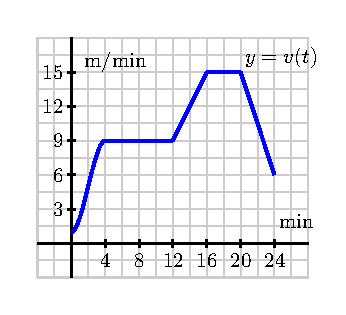
\includegraphics[scale=.75]{figures/4_4_Ez2.eps}
%
%    \ba
%  	\item Determine the exact distance traveled by the object on the time interval $0 \le t \le 4$.
%	\item What is the object's average velocity on $[12,24]$?
%	\item At what time is the object's acceleration greatest?
%	\item Suppose that the velocity of the object is increased by a constant value $c$ for all values of $t$.  What value of $c$ will make the object's total distance traveled on $[12,24]$ be 210 meters?
%  \ea
%  
%    \item When an aircraft attempts to climb as rapidly as
%possible, its climb rate (in feet per minute) decreases as altitude
%increases, because the air is less dense at higher altitudes.
%Given below is a table showing performance data for a certain
%single engine aircraft, giving its climb rate at various altitudes, where  $c(h)$ denotes the climb rate of the airplane at an altitude $h$.
%
%
%\begin{center}
%\scalebox{.85}{
%  \begin{tabular}{|c||c|c|c|c|c|c|}
%    \hline
%    $h$ (feet)&0&1000&2000&3000&4000&5000\\
%    \hline
%    $c$ (ft/min)&925&875&830&780&730&685\\
%    \hline
%    \hline
%    $h$ (feet)&6000&7000&8000&9000&10,000&\\
%    \hline
%    $c$ (ft/min)&635&585&535&490&440&\\
%    \hline
%  \end{tabular}
%  }
%\end{center}
%
%
% Let a new function called $m(h)$ measure
%the number of minutes required for a plane at altitude $h$ to climb the
%next foot of altitude.
%\ba
%	\item Determine a similar table of values for $m(h)$ and explain how it is related to the table above.  Be sure to explain the units.
%
%	\item Give a careful interpretation of a function whose derivative
%is $m(h)$.  Describe what the input is and what the output is.  Also,
%explain in plain English what the function tells us.
%
%	\item Determine a definite integral whose value tells us exactly the number of minutes required for the airplane to ascend to
%10,000 feet of altitude.  Clearly explain why the value of this integral has the required meaning.
%
%	\item Use the Riemann sum $M_5$ to estimate the value of the integral you found in (c).  Include units on your result.
%\ea
%
%
%\end{enumerate}
%
%%---------------------------------------------
%% END OF EXERCISES ON SECOND PAGE
%%---------------------------------------------
%\end{multicols*}
%\end{adjustwidth*}

\afterexercises 

\cleardoublepage
